\chapter{System Evaluation}

This chapter presents the evaluation of the system on test data.
Section~\ref{sec:eval:meth} would detail the evaluation methodology,
while Section~\ref{sec:eval:res} would provide some sample results.

\section{Evaluation Methodology}\label{sec:eval:meth}

This section focuses on two specific aspects of the evaluation methodology
--- the scope of functionality tested (and the system configuration applicable for
testing), and the data used in the evaluation.

\subsection{Scope of Evaluation}

Section~\ref{sec:im:code:sys} detailed the CLI for the system. Hence our evaluation
aims to test the two major functionalities of the system through the CLI\@:

\begin{itemize}
    \item System setup --- single, multiple or all modules
    \item System processing --- processing using each of the four pipelines
\end{itemize}

All 8 modules and 4 procedures implemented in Section~\ref{sec:im:code} will
be evaluated. 

\subsection{Data Used}

Testing will be done on one file object each, of the three multimedia data types
outline in Section~\ref{sec:in:back}. The details of the file objects are in
Table~\ref{eval-data}.

\begin{longtabu}{X[1,l]X[3,l]X[1,l]}
    \textbf{Data type} &
    \textbf{File description}
    & \textbf{File metadata} \\
    \midrule
    \endhead{}
    Single-file audio & 
    Singapore's 93.8FM\@: ``2017 Outlook on the Tech Start-up Scene
    in Singapore'' &
    \texttt{.mp3} file, 2m45s \\
    Single-file video &
    Singapore's Parliament proceedings: ``Minister Ng Eng Hen's response
    on the SAF's efforts to deal with terrorism threat'' &
    \texttt{.mp4} file, 1m58s \\
    Multi-channel recordings &
    SLRG recording of 4 male speakers on Singapore Army &
    \texttt{.wav} files, 2m00s\footnote{The original recording is 13m30s. The
    testing data is the first 2m00s that does not contain all 4 speakers.} \\
    \caption{Evaluation data}\label{eval-data}
\end{longtabu}

\newpage

\section{Evaluation Results}\label{sec:eval:res}

The results are briefly reported in the following sections.

\subsection{System Setup}

Figure~\ref{eval-1mod} shows a sample setup for one module.

\begin{figure}[ht]
\begin{lstlisting}
$ python system.py setup -m resample-1.0

2017-10-23 16:06:15,802 (system | INFO) : Starting setup...
Requirement already up-to-date: ffmpy in home/nhanh/.local/lib/python2.7/site-packages
2017-10-23 16:06:16,264 (system | INFO) : Setup successful for module resample-1.0
\end{lstlisting}
\caption{Sample setup for module \texttt{resample}}\label{eval-1mod}
\end{figure}

Figure~\ref{eval-2mod} shows a sample setup for multiple modules.

\begin{figure}[ht]
\begin{lstlisting}
$ python system.py setup -m visualize-1.0 capgen-1.0

2017-10-23 16:09:06,105 (system | INFO) : Starting setup...
Requirement already up-to-date: ffmpy in /home/nhanh/.local/lib/python2.7/site-packages
2017-10-23 16:09:06,564 (system | INFO) : Setup successful for module visualize-1.0
Torch already installed
nn scm-1 already installed
nngraph scm-1 already installed
image 1.1.alpha-0 already installed
lua-cjson 2.1.0-1 already installed
Required rocks installed
loadcaffe already installed
torch-hdf5 0-0 already installed
CPU checkpoints downloaded
2017-10-23 16:09:06,847 (system | INFO) : Setup successful for module capgen-1.0
\end{lstlisting}
\caption{Sample setup for modules \texttt{visualize} and
\texttt{capgen}}\label{eval-2mod}
\end{figure}

The two figures show a consistent setup process; and when individual setups are
successful, the status would be logged on screen, consistent with our system
implementation in Section~\ref{sec:im:code:log}.

\subsection{System Processing}

We are particularly interested in visualization of the transcripts and captions;
the sample output in Figure~\ref{eval-vid}~\footnote{Screen output sequences
shortened.} holds for the visualization process on the single video file in
Table~\ref{eval-data}.

The figure illustrates all the features of the implemented processing workflow
--- start-up manifest checks, file imports and file operations. The visualization
process in the current system does transcription by Google Cloud Speech API
before visualization; however as the transcription has been done before, the
whole transcription passes by as no-ops, and the behaviour logged appropriately.
Two transcripts and one keyframe captioning would be visualized, as shown in the
screen capture in Figure~\ref{eval-cap}.

\begin{figure}[ht]
\begin{center}
    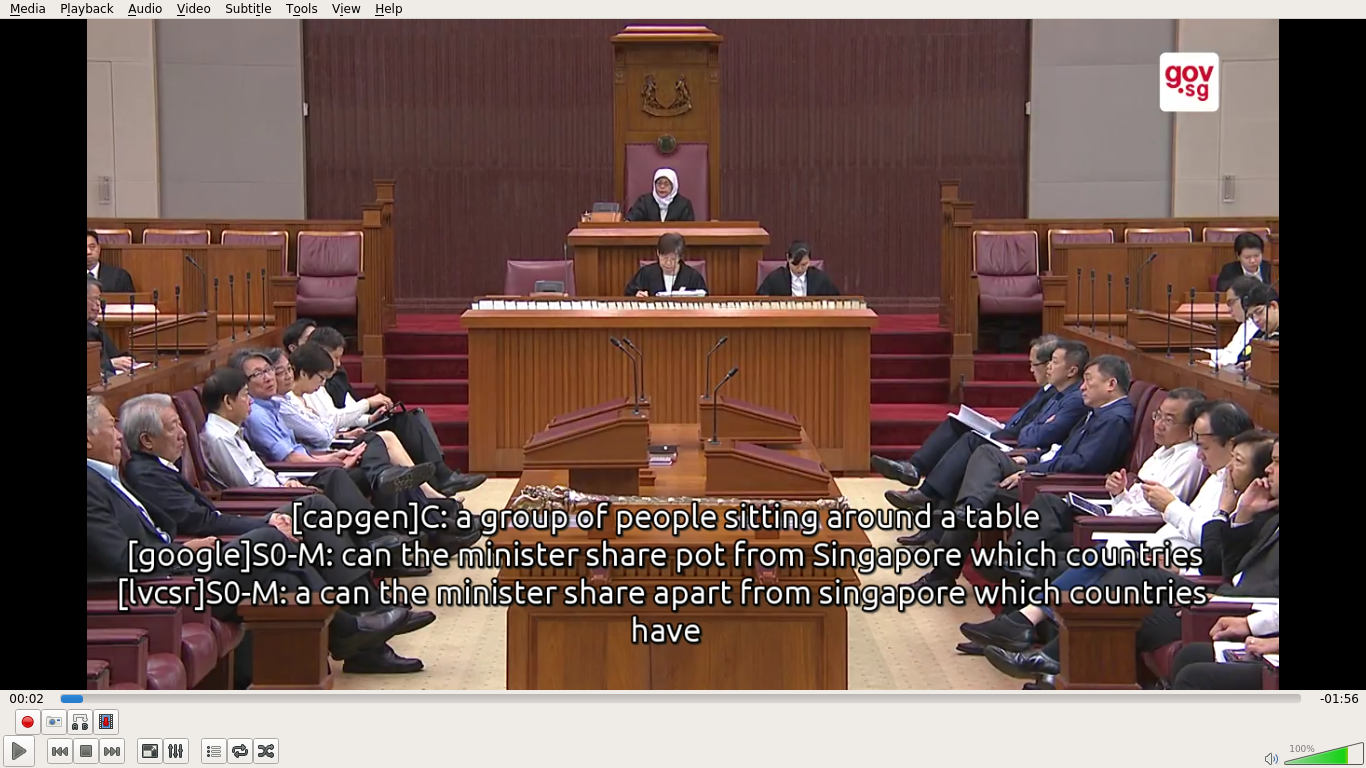
\includegraphics[width=\textwidth]{eval_caption}
    \caption{Screen caption of visualization}\label{eval-cap}
\end{center}
\end{figure}

\begin{figure}[ht]
\begin{lstlisting}
$ python system.py process process-1 -p visualize

2017-10-23 16:17:56,797 (system | INFO) : Loading manifests...
2017-10-23 16:17:56,898 (system | INFO) : Startup manifest checks...
2017-10-23 16:17:56,898 (system | INFO) : Valid modules: resample-1.0, capgen-1.0, lvcsr-1701, diarize-8.4.1, convert-1.0, google-1, vad-1.0, visualize-1.0
2017-10-23 16:17:56,898 (system | INFO) : Checking process process-1
2017-10-23 16:17:56,899 (system | INFO) : Valid procedures: capgen, google, lvcsr, vad, visualize

2017-10-23 16:17:56,917 (system | INFO) : Process: process-1
2017-10-23 16:17:56,917 (system | INFO) : Procedure: visualize
2017-10-23 16:17:56,917 (system | INFO) : Filename: Minister Ng Eng Hen's response on the SAF's efforts to deal with the terrorism threat.mp4
2017-10-23 16:17:56,917 (system | INFO) : File ID: minister-ng-eng-hen-s-response-on-the-saf-s-efforts-to-deal-with-the-terrorism-threat
2017-10-23 16:17:56,917 (system | INFO) : Previously imported to ...
2017-10-23 16:17:56,995 (resample | DEBUG) : Previously resampled ...
2017-10-23 16:17:57,076 (diarize | DEBUG) : Previously diarized to ...
2017-10-23 16:17:59,808 (google | DEBUG) : Transcribing single audio stream...
2017-10-23 16:17:59,808 (google | DEBUG) : Previously transcribed ...
2017-10-23 16:18:00,143 (visualize | DEBUG) : tg_to_srt operation previously completed for .../lvcsr/...TextGrid
2017-10-23 16:18:00,143 (visualize | DEBUG) : tg_to_srt operation previously completed for .../google/...TextGrid
2017-10-23 16:18:00,150 (visualize | DEBUG) : tg_to_srt operation previously completed for .../keyframes/...TextGrid
2017-10-23 16:18:00,152 (visualize | DEBUG) : combine_srt operation completed
2017-10-23 16:18:00,154 (visualize | DEBUG) : Written .../visualize/...srt
2017-10-23 16:18:00,154 (visualize | DEBUG) : Previously processed .../visualize/...mp4
2017-10-23 16:18:00,159 (system | INFO) : Pipeline completed for minister-ng-eng-hen-s-response-on-the-saf-s-efforts-to-deal-with-the-terrorism-threat using procedure visualize
\end{lstlisting}
\caption{Sample processing output}\label{eval-vid}
\end{figure}
